\documentclass[conference]{IEEEtran}
\usepackage[utf8]{inputenc}
\usepackage[modulo]{lineno}
\usepackage[numbers]{natbib}
\usepackage{url}
\usepackage{import}
\usepackage{tabularx}
\usepackage{graphicx}
\usepackage{comment}
\usepackage{bm}
\usepackage{hyperref}
\usepackage{caption}
\usepackage{subcaption}

% Macros for proof-reading
\usepackage[normalem]{ulem} % for \sout
\usepackage{xcolor}
\newcommand{\ra}{$\rightarrow$}
\newcommand{\ugh}[1]{\textcolor{red}{\uwave{#1}}} % please rephrase
\newcommand{\ins}[1]{\textcolor{blue}{\uline{#1}}} % please insert
\newcommand{\del}[1]{\textcolor{red}{\sout{#1}}} % please delete
\newcommand{\chg}[2]{\textcolor{red}{\sout{#1}}{\ra}\textcolor{blue}{\uline{#2}}} % please change

% Put edit comments in a really ugly standout display
\usepackage{ifthen}
\usepackage{amssymb}
\newboolean{showcomments}
\setboolean{showcomments}{true} % toggle to show or hide comments
\ifthenelse{\boolean{showcomments}}
  {\newcommand{\nb}[2]{
    \fcolorbox{gray}{yellow}{\bfseries\sffamily\scriptsize#1}
    {\sf\small$\blacktriangleright$\textit{#2}$\blacktriangleleft$}
   }
   \newcommand{\version}{\emph{\scriptsize$-$working$-$}}
  }
  {\newcommand{\nb}[2]{}
   \newcommand{\version}{}
  }

\newcommand\eric[1]{\nb{Eric}{#1}}
\newcommand\francisco[1]{\nb{Francisco}{#1}}
\newcommand\grischa[1]{\nb{Grischa}{#1}}
\newcommand\rebekka[1]{\nb{Jennifer}{#1}}
\newcommand\rashidah[1]{\nb{Rashidah}{#1}}
\newcommand\kurt[1]{\nb{Kurt}{#1}}

% Nice tables
\usepackage{booktabs}
\usepackage{array}
\usepackage{colortbl}
\usepackage{multirow}
\usepackage{longtable}


\newcolumntype{v}[1]{>{\raggedright \hspace {0pt}}p{#1}}
\newcolumntype{G}[1]{>{\columncolor{gray90}}#1}


%%%%%%%%%%%%%%%%%%%%%%%%%%%%%%%
 % New Colors: %%%%%%%%%%%%%%%%%
\definecolor{Gray}{gray}{0.8}
\definecolor{gray25}{gray}{0.25}
\definecolor{gray50}{gray}{0.50}
\definecolor{gray75}{gray}{0.75}
\definecolor{gray90}{gray}{0.9}


\newcommand{\grayrow}{\rowcolor{gray90}}
\newcommand{\interviewquote}[2]{\begin{quote}
\footnotesize{\emph{``#1'' }} --- \footnotesize{#2}
\end{quote} }

\title{Quality Requirements in Agile as a Knowledge Management Problem: More than Just-in-Time%\\ \Large{--Position Paper--}
}

\author{
\IEEEauthorblockN{Eric Knauss, Grischa Liebel}
\IEEEauthorblockA{Computer Science and Engineering\\
Chalmers $\mid$ University of Gothenburg \\ Gothenburg, Sweden \\ \{knauss,grischa\}@chalmers.se }
\and
\IEEEauthorblockN{Kurt Schneider}
\IEEEauthorblockA{Software Engineering Group\\
Leibniz Universit\"at Hannover \\ Hannover, Germany \\ ks@inf.uni-hannover.de}}

\begin{document}
\maketitle

\begin{abstract}
%\eric{very drafty, to set the scene}
Just-in-time (JIT) approaches have been suggested for managing non-functional requirements in agile projects.
However, many non-functional requirements cannot be raised and met on the spot. 
In this position paper, we argue that effective JIT engineering of quality requirements depends on a solid foundation of long-term knowledge  about all relevant quality requirements.
We present two examples from projects related to safety and security and show that not all aspects of these quality requirements can be invented and changed just in time. 
% Different roles and different stakeholders are responsible, and the tasks at hand determine how they can be handled. 
Further, managing for example operationalization of quality requirements just in time depends on sufficient understanding of (i) customer value and (ii) the system under construction that must be shared by the engineering team.
%
%Thus, it is not sufficient to focus on JIT requirements engineering alone. 
If a Learning Software Organization (LSO) intends to increase agility and speed up system development, it needs a holistic concept for managing this knowledge. 
%The assumed co-existence of JIT and solid non-functional requirements needs a structure for eliciting, storing, and managing quality requirements. 
%We claim that JIT management of quality requirements must be complemented by a long-term perspective.
We propose that a knowledge-management framework can facilitates JIT-RE by structuring, representing, and allowing updates of long-term knowledge about quality requirements.
Such a knowledge-management framework should allow to map user value to system requirements and have important properties to allow JIT RE and sustainable evolution. 
%We discuss properties of , by allow providing knowledge management structures and counterparts to represent – and update – the knowledge aspect of non-functional requirements.      \kurt{Which properties of the framework are important so that it supports JIT and sustainable evolution?}

\end{abstract}

\begin{IEEEkeywords}
just-in-time RE, quality requirements, managing requirements knowledge
\end{IEEEkeywords}

\section{Introduction}

%\eric{4pages! title, abstract, intro to finish on page 1}

% \eric{Abstract, Intro: Basic assumption JIT+long-term; this is a KM problem}


%\eric{Context: More and more system development companies are turning towards agile...}
In this position paper, we argue based on our experience in several projects that while just-in-time management of quality requirements is important in agile development, it must be complemented by an initiative to manage long-term aspects of quality requirements and to build and use knowledge about the system under construction.


%Agile approaches have significantly changed the way software is developed \cite{Meyer2014}.
%Based on reports of successes with small teams \cite{Meyer2014,kahkonen2004agile,beck2000extreme,paasivaara2016challenges}, these approaches are more and more applied in large scale \cite{dikert2016challenges,lagerberg13,salo2008agile} and in system development \cite{eklund14,berger15,lagerberg13}, an environment that is characterized by long lead times \cite{berger15} and stable, sequential engineering practices \cite{pernstal12}.

%\eric{Quality requirements have JIT and long-term aspects and we cannot support one without knowing about the other. A holistic knowledge management approach is needed.}

Agile software development lacks systematic approaches for managing quality requirements \cite{inayat2015systematic} and needs further research, even though a variety of promising practices for managing quality requirements are known \cite{Alsaqaf2017}. 
Among those, some relate to just-in-time aspects of quality requirements engineering: relying on face-to-face communication and iterative emergence of requirements \cite{Alsaqaf2017}. 
Others imply a long-term perspective on quality requirements, as for example product grooming, continuous integration, and test-driven development \cite{Alsaqaf2017}.
Yet, existing challenges of managing quality requirements in agile development show an inability to synchronize just-in-time RE activities and long-term perspectives on architecture and system verification. 
This is concerning: on the one hand, we need just-in-time analysis of quality requirements to operationalize them for functionality currently under development.
On the other hand, quality requirements can be considered long-term business drivers that allow diversification from competitors \cite{BerntssonSvensson2015}.
A%s Cockburn argues, a
n agile team not only needs to care about the current %game (i.e. the current
release or project%, the current project)
, but also about the next %game
\cite{Cockburn2009}.

\textbf{Proposition 1} (JIT vs. Long-Term): \emph{We propose that JIT management of quality requirements must be complemented by an initiative to manage long-term aspects of quality requirements.}
%
% \eric{Agile System Development needs a user value and a system understanding perspective. This is based on \cite{Kasauli2017a}.}
%
In agile requirements engineering, a lot of emphasis is on understanding and communicating customer and end-user value \cite{Alahyari2016}.
This is important, since agile approaches rely on self-organized teams with some autonomy \cite{Meyer2014} and these teams need to understand what provides customer value, before they can make decisions \cite{Kasauli2017}.
Pre-agile approaches to requirements engineering emphasize the importance of distinguishing between user requirements and system requirements \cite{Sommerville2006} and this importance has been confirmed for requirements engineering in large-scale agile system development \cite{Kasauli2017a}. Incremental agile development and continuous delivery do not only require an excellent understanding of customer value, but also effective knowledge about how and why the current system was built. 

Consequently, many challenges in agile management of quality requirements relate to a lack of consideration of this system perspective in agile development, e.g. %\emph
{focusing on delivering functionality at the cost of architecture flexibility} as well as %\emph
{ignoring predictable architecture requirements} \cite{Alsaqaf2017}. 

\textbf{Proposition 2} (Customer value vs. System knowledge): \emph{ We claim that both JIT and long-term management of quality requirements must consider both a user (or: market) value perspective and a system requirements perspective.}
%
We argue that most qualities cannot be significantly improved just-in-time. 
While for example a single change can destroy security or safety of a system, the only way to create a system that has these properties is to grow it around a strong notion of the most important qualities. 
The knowledge how this has been done must be conserved and must be made accessible for JIT quality requirements activities.

In this position paper, we revisit well established knowledge management literature with our two key propositions in mind.
 

%In the following Section, we discuss foundations of knowledge management and how they relate to requirements engineering. In Section 3, we discuss the aspects and constraints of a suitable knowledge management framework for quality requirements in agile. 
%By this, we hope to enable more research on this important topic and discuss implications for future research in Section 3.

%\begin{itemize}
%    \item NEW: There exist different schools of knowledge management and we can conclude that there are alternatives to a technocratical, database centric approach. Behavioral and business perspectives are important in agile. (argue with EKSE book,  p60)
%  \item NEW: Business value in agile methods does very well fit into this view.
%
% \end{itemize}
\section{Knowledge Management Foundations for Managing Quality Requirements}

In this paper, we consider requirements engineering as a knowledge management problem. 
Knowledge management addresses the acquisition of knowledge, transforming it from tacit or implicit into explicit knowledge and back again, storing, disseminating, and evaluating it systematically, and applying it in new situations \cite{Schneider2009}.
We see requirements as a special type of knowledge, which needs to be managed in an organization.
Doing requirements engineering then relates to organizational learning, which is an approach that stimulates learning of individuals, organization-wide collection of knowledge, and cultivation of infrastructure for knowledge exchange \cite{Schneider2009}.


%\eric{Classic KM, RBS, Cockburn...}

%\begin{itemize}
%\item Usabilty/security/safety: qualities differ, also their JIT behavior.
%\item Doors as a requirements database, a knowledge base of an LSO
%\end{itemize}

Nonaka's and Takeuchi's theory of knowledge creation relates to tacit and explicit knowledge \cite{Nonaka1995}\footnote{note that their notion of tacit knowledge differs from how this term is usually used in RE research: for them, tacit knowledge is not explicitly documented but can be shared in face-to-face communication.}.  
%
%We consider requirements engineering a crucial, knowledge generating activity.
Knowledge is created by converting it from a knowledge source (either tacit or explicit) to a new knowledge store (also either tacit or explicit). 
This view relates very well to requirements management, especially for quality requirements. 
For example, conversion of tacit knowledge to tacit knowledge (\emph{socialization} in Fig. \ref{fig:nonaka1995}), corresponds to an agile way of managing requirements, that de-emphasizes documentation and instead relies on face-to-face communication and just-in-time clarification of requirements. 
A long-term perspective on requirements would require explicit knowledge representations.
\emph{Combination}, for example, corresponds to tracing information derived from relating different artifacts of system engineering to each other. 
%Thus, we are especially interested in Nonaka's and Takeuchi's works on conversion between tacit and explit knowledge representations, as depicted in Fig. \ref{fig:nonaka1995}.

Earl has developed a framework to classify studies on knowledge management according to different research directions, which he calls schools \cite{Earl2001}.
The \emph{technocratic} school focuses on systems, maps and engineering of knowledge and resonates with a traditional approach to requirements engineering with a central requirements database (or specification) as knowledge base. 
In contrast, the \emph{economic} school focuses on commercial value of knowledge and the \emph{behavioral} school considers organizational, spatial, and strategic aspects.
We note that these latter schools resonate with values of agile RE.
\section{Example 1: Safety}

Safety can be briefly characterized as the confidence that a software or technical system will not harm humans or cause major damage or financial loss. Airplanes or cars need to ensure functional safety according to ISE 61 508 or ISO 26262. An autonomous driving system must ensure that the intelligent breaks will not cause accidents.

\begin{figure}[t]
    \centering
    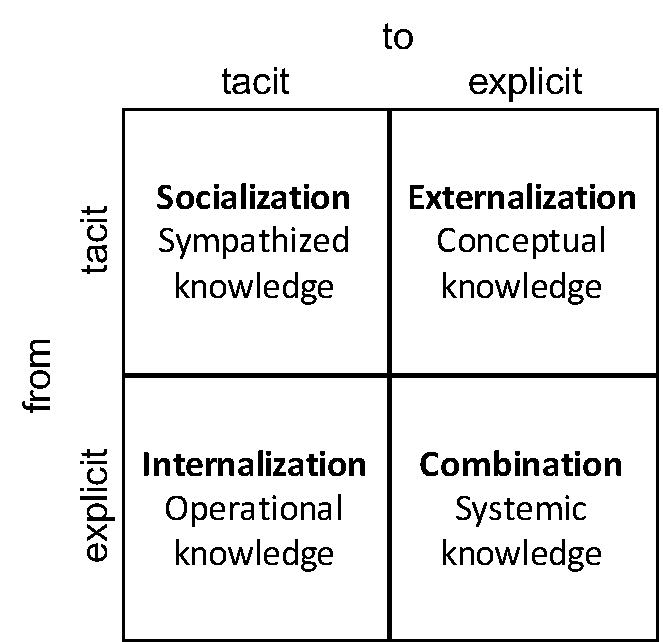
\includegraphics[width=0.5\columnwidth]{figs/nonaka95}
    \caption{Conversions between tacit and explicit knowledge \cite{Nonaka1995}.}
    \label{fig:nonaka1995}
\end{figure}

In our project on Requirements Engineering for large-scale agile system development \cite{Kasauli2017a}, many case companies develop safety critical systems and are subjected to regulation. 
These companies struggle to establish an effective approach to manage safety that still supports agile, incremental work. 
Regulations often require comprehensive tracing information that relates different system engineering artifacts to each other and allows to show how safety was systematically build into the system.
Further, %verifying the safety of large-scale systems takes significant resources and time.
%In 
in order to support incremental, agile development, it is desirable to also allow for incremental verification. 
For this and other reasons, safety must already be considered during creating the system architecture, e.g. by defining independent components, separating safety concerns from others, and provide redundancies for critical components.
This requires long term system knowledge, mainly created through \emph{combination} (Fig. \ref{fig:nonaka1995}) of existing system artifacts.

Yet, there is always a risk to include a change %to the system 
that effectively declines the safety of a component.
This risk must be mitigated just-in-time, for example by doing a change-impact-analysis to understand which components will be affected and then \emph{internalize} the existing knowledge about the system under construction.
In our experience, practitioners often reach out to domain experts to help them assess the system requirements efficiently, leading to emergent collaboration.

When a cross-functional team starts the development of a new feature for a safety critical system, one of the first steps is to do a hazard analysis. 
The result will inform the team about the safety criticality of the feature, which in turn defines the engineering method to be applied. 
This activity can be considered to be just-in-time and relies on \emph{internalization} of existing system knowledge as well as on \emph{socialization} to discuss how the feature will affect functional safety.% of users and other stakeholders. 

The foundation for such reasoning is long-term knowledge about the desired (or required) level of safety. 
While this knowledge might have been established at one time face-to-face through socialization of domain experts, it is long-lasting and reusable (i.e. the next product will relate to very similar safety concerns). 
Thus, an efficient way of \emph{externalization} of this knowledge is required. 

Today, this externalization is not emphasized in many agile system development approaches.
Due to the long-lasting nature of safety considerations of systems, existing documentation can be reused after a company has transitioned from v-model or waterfall approaches to agile. 
However, we argue that updating and maintaining this knowledge must be considered in any approach to agile system development.
\section{Example 2: Security}

Security is defined as the ability of a system to withstand attacks. 
In contrast to safety, security does assume an adversary viciously attacking the software. 
%Being able to protect a system against attacks requires 
Developers need to anticipate and consider all potential attacks; in misuse-cases \cite{Alexander2002a}, this antagonism between two sides is made explicit. This \emph{externalization} is often supported by attack trees.%, which help developers to consider all possible attacks.

Knowledge about vulnerabilities, past attacks, and many other aspects of a software system is crucial for both sides. 
If developers want to stay ahead of attackers, they need to organize and use that knowledge. 
In the German DFG Priority Programme 1593 (Design for Future), we work on an approach for detecting vulnerabilities during requirements analysis. 
This ``SecVolution'' approach is fundamentally built on a knowledge-perspective of security \cite{Gaertner2014,fosad14}. 

Security is a quality aspect of growing importance: Large home entertainment systems may have been initially out of scope for security, but when they collect payment information or personal data, they suddenly become very security-relevant. 
Supermarket management software may start out as a local and non-distributed application of moderate size and limited security relevance. 
When an online-store component is added, software security definitely turns into a major concern. 
As these examples indicate, security is far from a commodity that can be added and removed at convenience. 
Instead, a single known vulnerability can make the entire system insecure. 
SecVolution investigates changes that can cause security to suffer. 
The above-mentioned scenarios exemplify this type of changes. 
However, there is an additional type of changes that is not mentioned above but just as severe: Even if nothing in the software changes, its security can suffer when attackers discover a new security breach in the existing code, and exploit it for an attack. 
A long-living system does not wear out over time, but it ages in relationship to the knowledge developers and attackers have about it. 
A core insight in SecVolution was how crucial it is to \emph{externalize} attacker and security knowledge from people; automate it in a tool, and help developers internalizing it when they see suspicious findings.


%Fig. Prinzipbild von SecVol
\begin{figure}
    \centering
    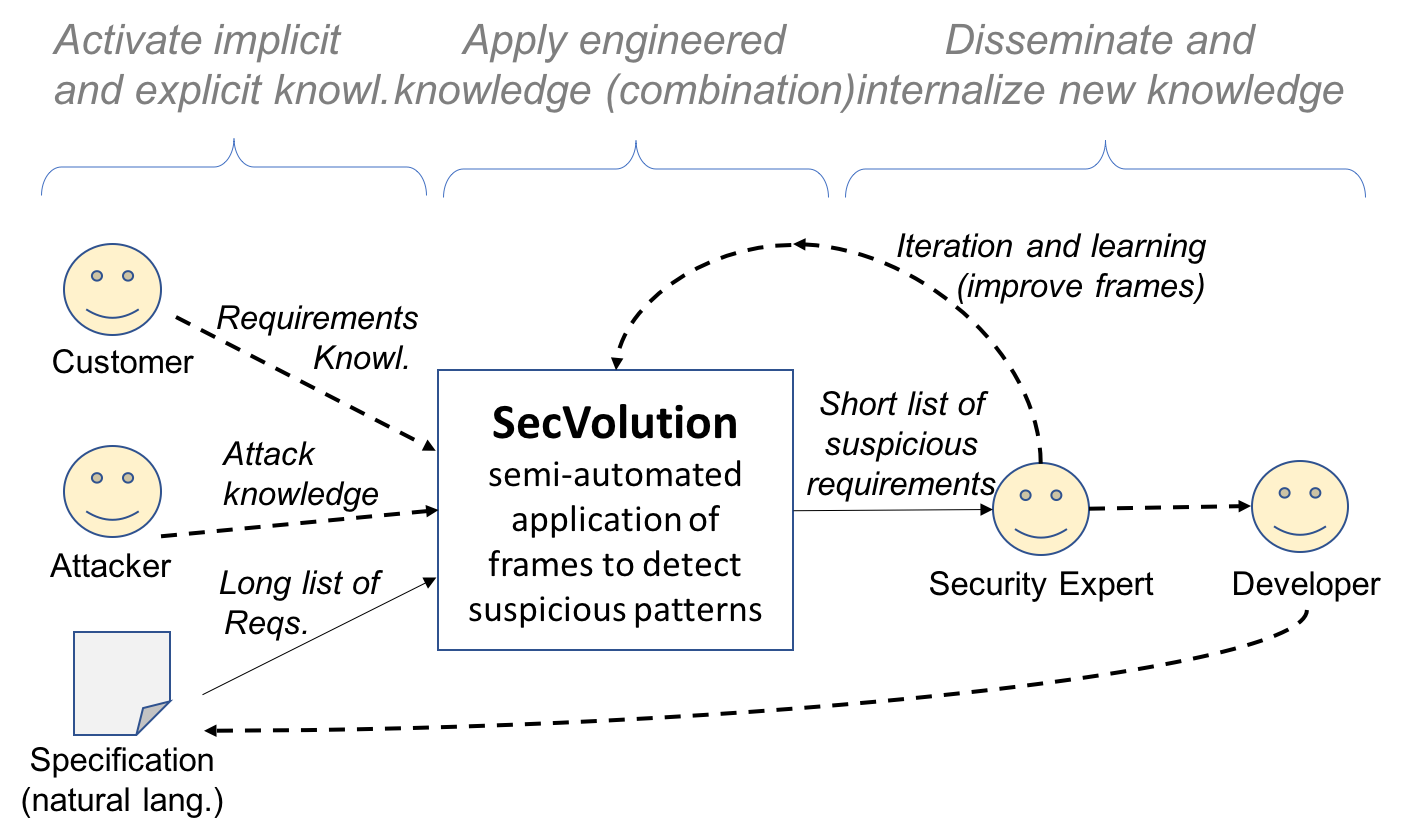
\includegraphics[width=\columnwidth]{figs/nnnOben}
    \caption{Three essential activities in managing knowledge on software quality attributes.}
    \label{fig:nnnOben}
\end{figure}

%We wanted to detect requirements that could introduce vulnerabilities. 
Highly qualified security experts are able to spot patterns of payment, data, access, and the like. 
However, those experts are rare and cannot check each and every document and use case. 
A presumably unproblematic system, such as a supermarket or smart TV, tends to be neglected in terms of security. 
Thus, SecVolution tries to detect as many known suspicious requirements and submit this much smaller list of requirements to the rare experts for final resolution. 
In order to extract knowledge from human-made natural language requirements, we use natural-language processing techniques. 
% About 79\% of requirements are still in natural language. 
After parsing the sentence grammatically, we search for matching Security Frames (i.e., suspicious patterns) and use an ontology to represent the knowledge. 


Techniques for soliciting and deriving explicit knowledge from  people who have internalized it can be very challenging \cite{Gaertner2014}. 
% Adding a new suspicious pattern to the heuristics could be done just in time. 
As a prerequisite, the %long-term 
collection of knowledge must be maintained as a long-term endeavor and the interplay of developers, attackers, and security experts must be investigated. 

\section{Towards a KM Framework}

%Constraints for such a framework, add two examples as boxes.


\begin{figure}
    \centering
    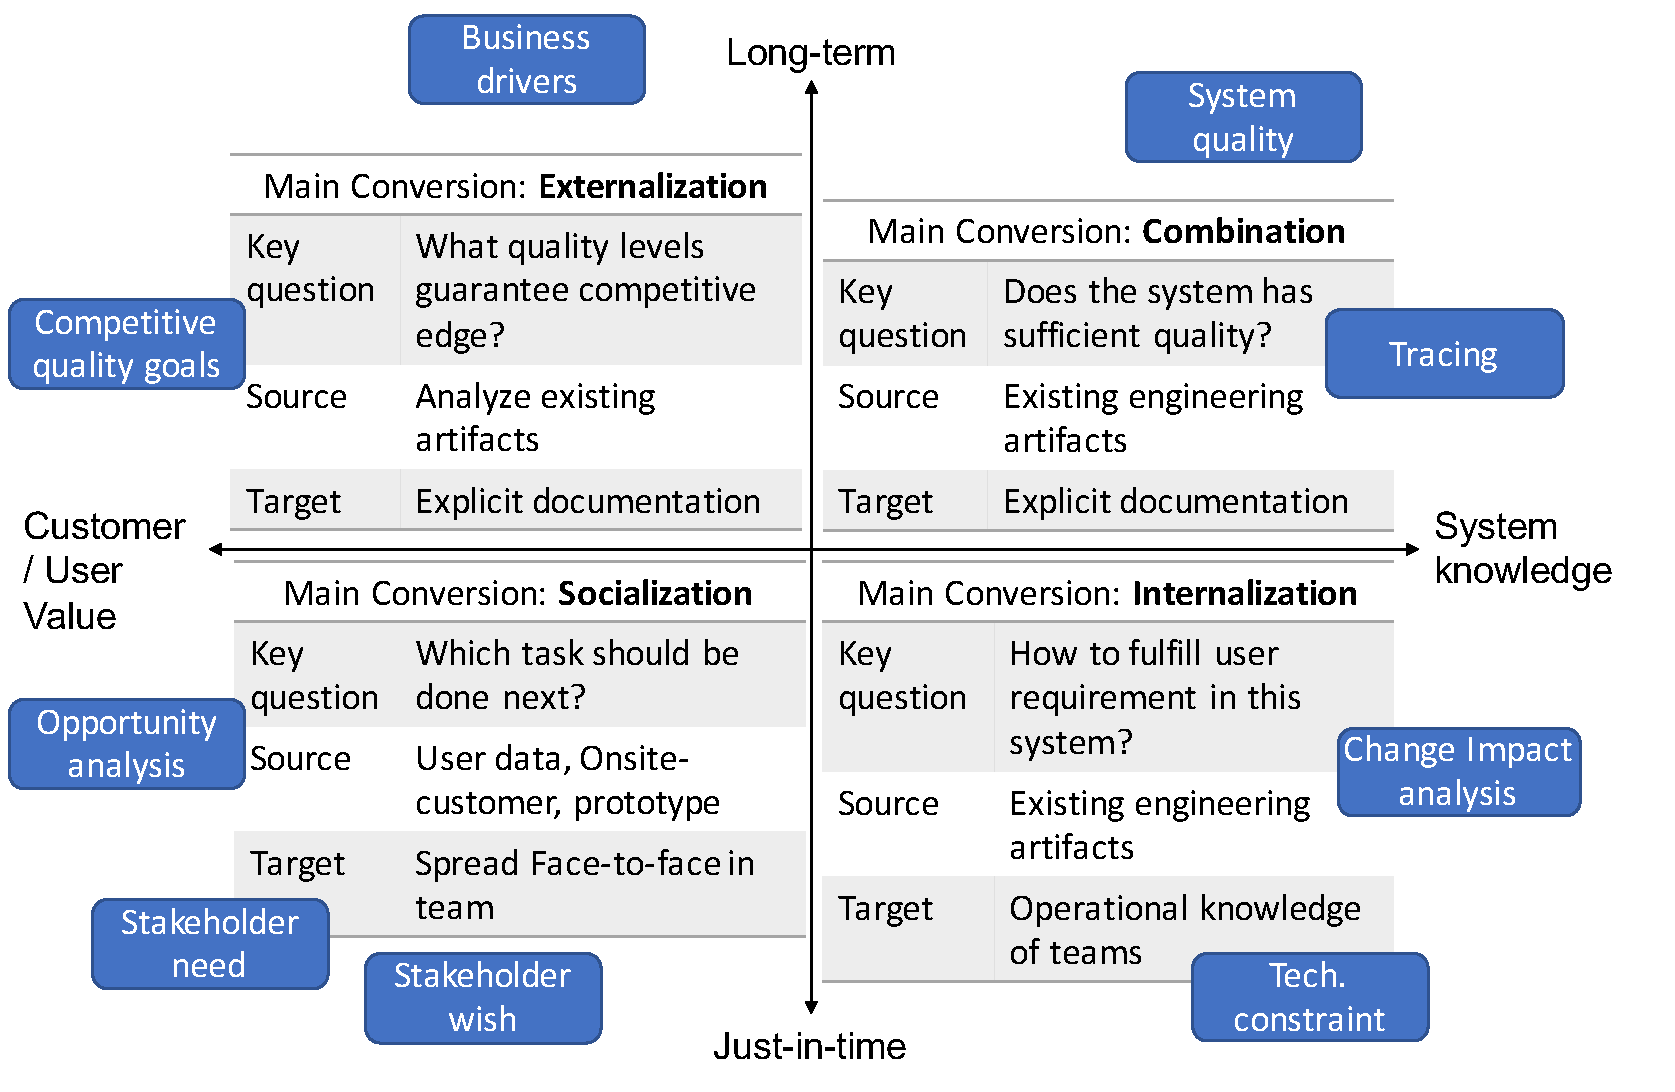
\includegraphics[width=\columnwidth]{figs/km-framework}
    \caption{Towards a Knowledge Management Framework for Agile Quality Requirements Management: Aligning knowledge conversion with our propositions.}
    \label{fig:km_conversion}
\end{figure}




Safety and security are two quality requirements that cannot be managed purely JIT. Quality requirements are typically related to architecture %, whereas functional requirements influence data structures, algorithms, and design patterns. 
%As we have pointed out above, quality requirements
and tend to build on knowledge as much as on software structures, although both need to come together.

In the above-mentioned SecVolution case, an ontology plays a central role of managing knowledge. %The input to that ontology comes from earlier experiences (of attacks), external published warnings (of vulnerabilities), and from insights of security experts. 
Earlier experiences (of attacks), external published warnings (of vulnerabilities), and  insights of security experts are encoded in the ontology, which can then be applied  %, the security frames etc,
%it can be applied 
to natural-language  requirements (Fig. \ref{fig:nnnOben}). 


There are obvious technical challenges involved in building such a knowledge infrastructure. It turned out to be at least equally challenging to solicit, interpret, and engineer the knowledge. Initially, most of that knowledge resides in people and needs to be externalized \cite{Nonaka1995} before it can be encoded and stored in an ontology. Therefore, extracting implicit or even tacit knowledge from people is one of the focus areas within SecVolution. This step is essential and not just a side-issue. Similar to the experience reported in \cite{Schneider2009}, tapping human knowledge and experience is almost a discipline by itself. Making a knowledge management infrastructure effective requires taking the social and socio-technical challenges seriously. The central part in Fig. \ref{fig:nnnOben} is the technological infrastructure for managing explicit knowledge. Schneider presents an experience life cycle\cite{Schneider2009} in software engineering: Activation and collection are  devoted to techniques and tools for attracting implicit or tacit knowledge into the system. For example, the by-product approach has been used for soliciting experience as a by-product of other tasks that need to be conducted anyway \cite{Schneider2006}. A purely technocratic view \cite{Earl2001} tends to neglect the left-hand input block. Along the same lines, many experiences (or knowledge items collected) are never actively disseminated. Thus, they remain useless.


%\ugh{Fig: der Kreis mit dne vier Aktivitäten rund um den Computer: siehe figs.pptx.    }

\begin{figure}
        \centering
    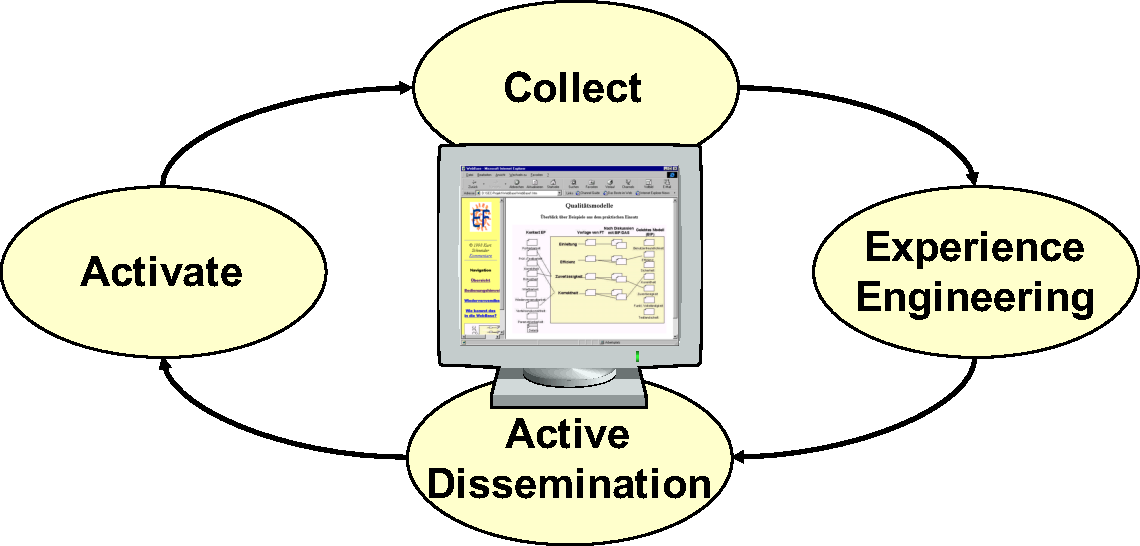
\includegraphics[width=0.7\columnwidth]{figs/nnnUnten}
    \caption{Life-cycle of experiences, iterating around experience base.}
    \label{fig:nnnUnten}
\end{figure}


Experts need to be made aware of the valuable knowledge they have (activate); there must be support to collect that information once it surfaces (collect, e.g. as a by-product \cite{Schneider2006}). Usually, the knowledge cannot be collected in exactly the same form that is most appropriate for reuse. Following Basili’s \cite{Basili1994} terminology, we call the activity of merging, comparing, and reformatting ``experience and knowledge engineering''. Finally, the resulting knowledge must be delivered to where it is needed, when it is needed, and in the most adequate form. In the SecVolution example, knowledge ends up in an ontology and is automatically applied to natural-language requirements. This is a very clear and technically sophisticated way of distribution. In other cases, knowledge will need to be presented to developers, requiring them to understand and apply it (e.g., for performance requirements).

Figures \ref{fig:km_conversion} and \ref{fig:nnnUnten} sketch the core of a knowledge management infrastructure for quality requirements: Fig \ref{fig:nnnUnten}  stresses the iterative nature of experience or knowledge about a quality aspect. Such an iterative process is applicable to JIT as well as to stiff and long-term requirements. Fig. \ref{fig:km_conversion} highlights different types of sources and the knowledge operations conducted. %JIT requirements for mitigating a new vulnerability if (and only if) security was continuously maintained. 
JIT and long-term requirements are not a contradiction, but need to complement each other.



%\section{Conclusion and Outlook}

%Some research roadmap perhaps?

\textbf{Acknowledgments.}
This work was supported by  Software Center (RE for Large-Scale Agile System Dev. Project) and German DFG Priority Programme 1593 (Design for Future).

\bibliographystyle{plainnat}
\bibliography{jit-as-km-problem.bib}
\end{document}